\chapter{Results}
%A measurement of two-neutron opening angle distributions in the photofission of $^{238}$U
%using Bremsstrahlung photons produced via a low duty factor, pulsed LINAC, is complete.
%These results confirm the expected dependency of neutron coincidence rate on opening angle and mean neutron energy.
%Figure~\ref{fig:result} includes the coefficients from a least-squares best-fit of the data to a second order Legendre polynomial.
%These coefficients, $a_0$ and $a_2$, are a measure of the isotropic and dipole components of the opening angle distributions, respectively.
%\begin{figure}
%    \centering
%    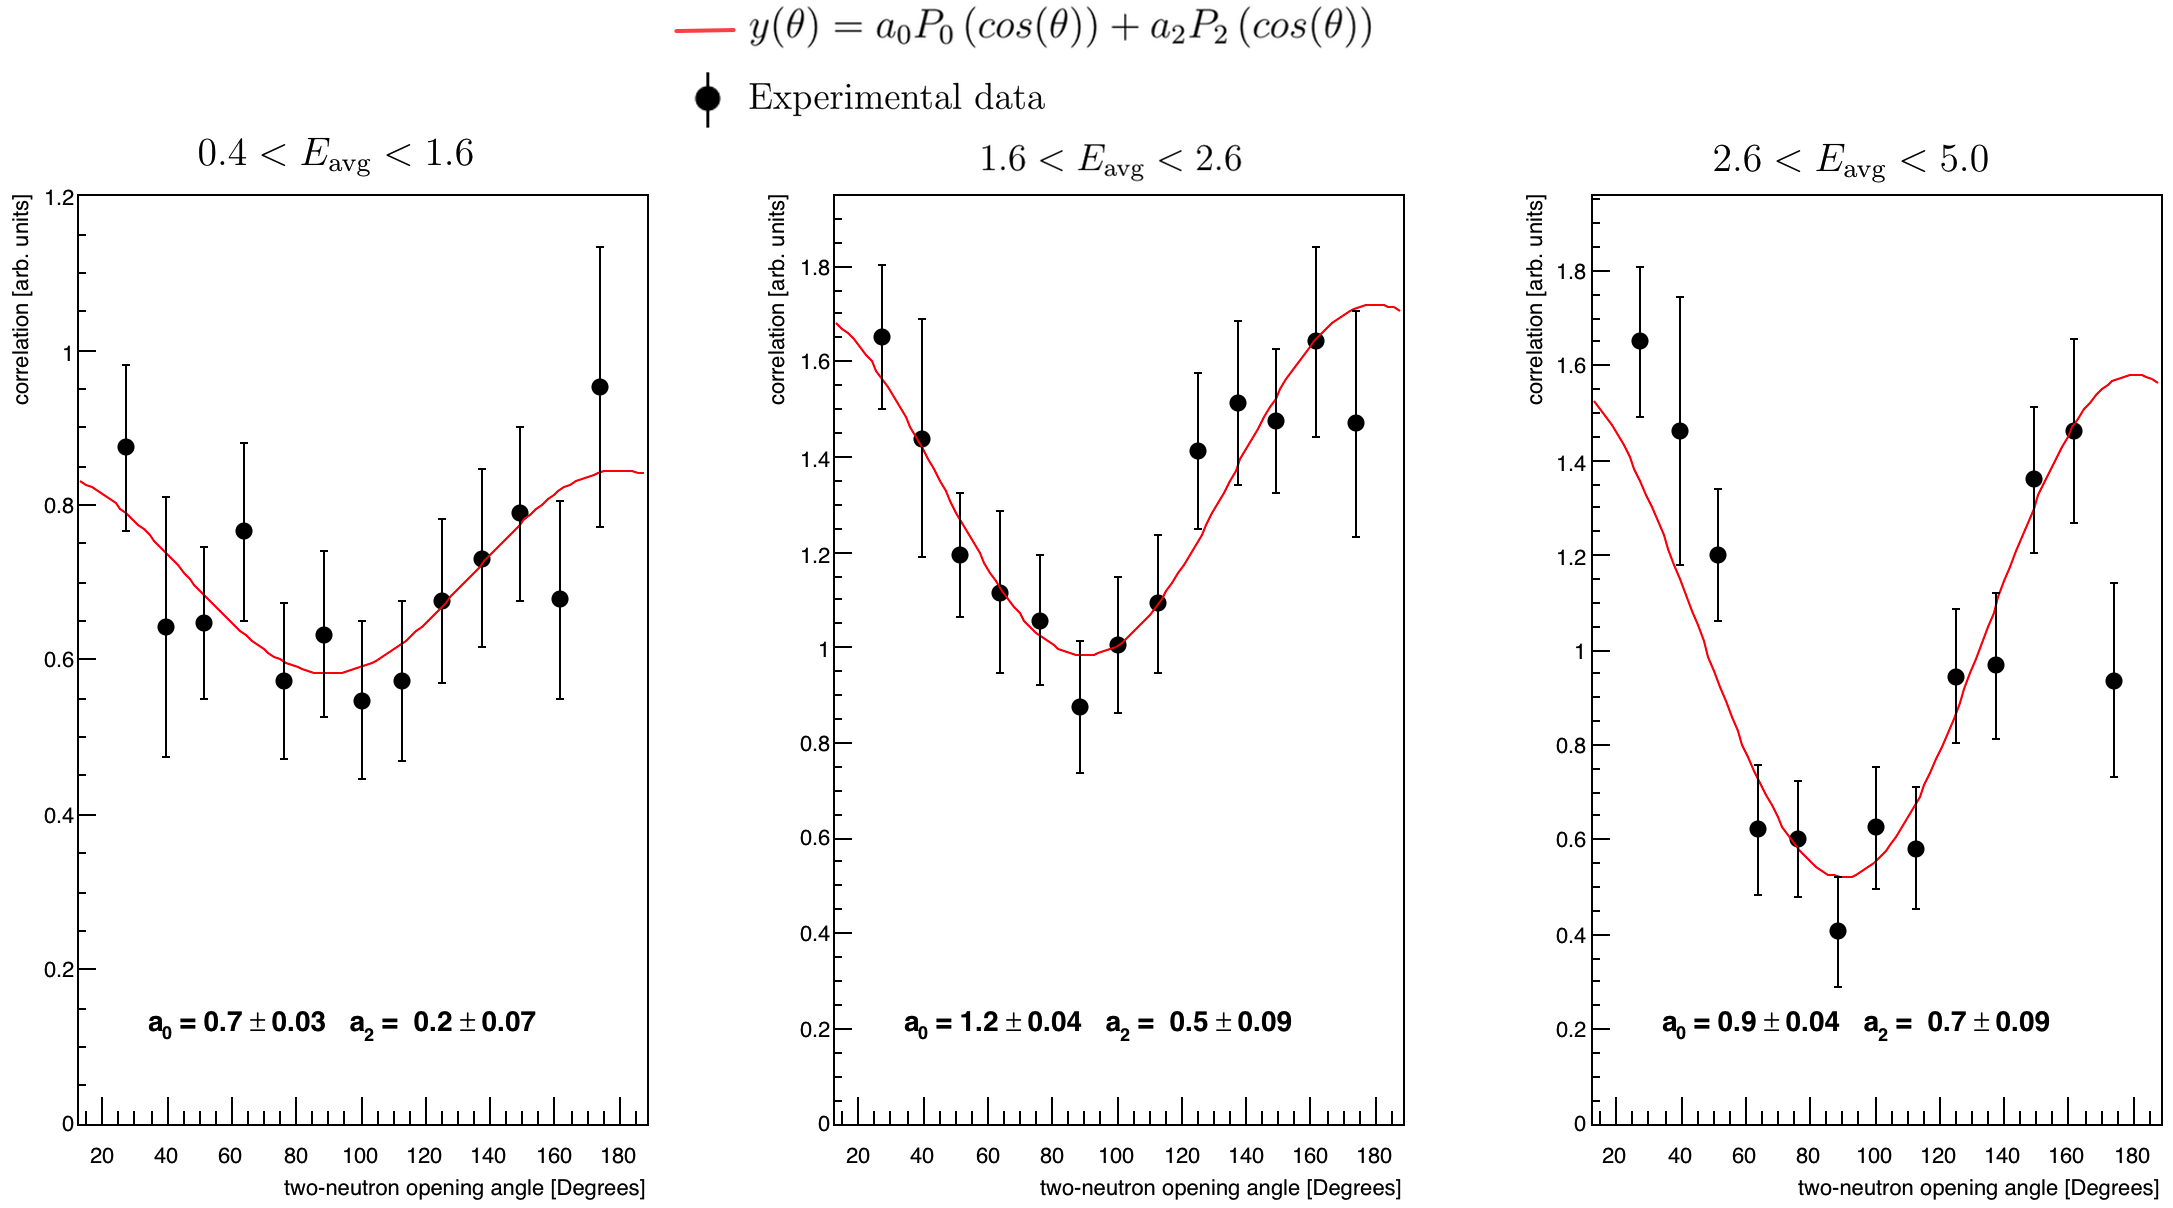
\includegraphics[width =\textwidth]{Content/Results/result.png}
%    \caption{Preliminary results of two-neutron opening angle distributions for three different average neutron energy ranges (energy range at top of each plot).
%    The coefficients of a best-fit to a 2$^{nd}$ order Legendre polynomial appear at the bottom of each plot.
%    }
%    \label{fig:result}
%\end{figure}